\documentclass[11pt,a4paper]{report}

% --- Core System Packages ---
\usepackage[utf8]{inputenc}
\usepackage[T1]{fontenc}
\usepackage[english]{babel}
\usepackage{amsmath, amssymb, amsfonts, amsthm}
\usepackage{graphicx}
\usepackage{geometry}
\geometry{top=0.7in, bottom=0.7in, left=0.7in, right=0.7in, headheight=15pt}
\usepackage{setspace}
\setstretch{1.1}
\usepackage{titlesec}
\usepackage[bookmarksopen=true,bookmarksnumbered=true]{hyperref}
\usepackage{xcolor}
\usepackage{booktabs}
\usepackage{array}
\usepackage{caption}
\usepackage{fancyhdr}
\usepackage{longtable}
\usepackage{multicol}
\usepackage[most]{tcolorbox}
\usepackage{tikz}
\usetikzlibrary{shapes.geometric, arrows, positioning, calc, shadows, backgrounds, fit}
\usepackage{enumitem}
\usepackage{microtype}
\usepackage{placeins}
\usepackage{float}
\usepackage{listings}
\usepackage{tabularx}
\usepackage{footnote}

% --- Custom Color Palette ---
\definecolor{agrigreen}{RGB}{0, 102, 51}
\definecolor{techblue}{RGB}{0, 51, 102}
\definecolor{acadred}{RGB}{139, 0, 0}
\definecolor{softgray}{RGB}{248, 248, 248}
\definecolor{boxblue}{RGB}{235, 245, 255}
\definecolor{boxgreen}{RGB}{240, 250, 240}

% --- Hyperlink Setup ---
\hypersetup{
    colorlinks=true,
    linkcolor=techblue,
    citecolor=agrigreen,
    urlcolor=acadred,
    pdftitle={AgriDecision-TN: High-Depth Academic IT Report},
    pdfauthor={Takwa Dalensi}
}

% --- Code Listing Style ---
\lstset{
    backgroundcolor=\color{softgray},
    basicstyle=\ttfamily\scriptsize,
    breaklines=true,
    frame=single,
    numbers=left,
    numberstyle=\tiny\color{gray},
    keywordstyle=\color{techblue},
    commentstyle=\color{agrigreen},
    stringstyle=\color{acadred},
    captionpos=b,
    xleftmargin=1.5em,
    framexleftmargin=1em
}

% --- Compact Box Designs ---
\newtcolorbox{itbox}[1]{%
    colback=boxblue, colframe=techblue, fonttitle=\bfseries\small,
    title={\textcolor{white}{#1}}, boxrule=0.5pt, arc=2pt, 
    left=6pt, right=6pt, top=4pt, bottom=4pt,
    enhanced, drop shadow
}

\newtcolorbox{techdetail}[1]{%
    colback=white, colframe=agrigreen, fonttitle=\bfseries\scriptsize,
    title={\textcolor{white}{#1}}, boxrule=0.3pt, arc=1pt,
    left=4pt, right=4pt, top=2pt, bottom=2pt
}

% --- Header/Footer Configuration ---
\pagestyle{fancy}
\fancyhf{}
\renewcommand{\headrulewidth}{0.1pt}
\lhead{\scriptsize \textcolor{agrigreen}{\textbf{AgriDecision-TN: High-Depth Academic IT Report}}}
\rhead{\scriptsize \textcolor{techblue}{T. Dalensi}}
\cfoot{\small\thepage}

% --- Chapter/Section Formatting ---
\titleformat{\chapter}[display]
  {\normalfont\Large\bfseries\color{agrigreen}}
  {\filleft\chaptertitlename\ \thechapter}{0pt}{\Large\filright}
\titlespacing*{\chapter}{0pt}{-10pt}{15pt}

\titleformat{\section}
  {\normalfont\large\bfseries\color{techblue}}
  {\thesection}{0.5em}{}

\titleformat{\subsection}
  {\normalfont\normalsize\bfseries\color{agrigreen!80!black}}
  {\thesubsection}{0.5em}{}

\begin{document}

% ============================================
% TITLE PAGE
% ============================================
\pagenumbering{roman}
\begin{titlepage}
    \centering
    \vspace*{1cm}
    {\Huge\bfseries\color{agrigreen} AgriDecision-TN}\\[0.5cm]
    {\Large\color{techblue}\textbf{Prescriptive Web Services \& Bayesian Architecture for Tunisian Agronomy}}\\[1cm]
    
    \begin{center}
        \includegraphics[width=0.45\textwidth]{uploaded_image_1768647956960.png} \\
        \footnotesize Figure 1: High-Level System Lifecycle
    \end{center}
    
    \vspace{0.8cm}
    \begin{itbox}{Abstract}
        \small This report presents the design and implementation of \textbf{AgriDecision-TN}, a multidimensional digital platform dedicated to the prescriptive support of Tunisian smallholder farmers through the digitalization of intangible agrarian heritage. In the contemporary environment of rapid climate change, traditional planting calendars are increasingly detached from actual bioclimatic realities—a phenomenon defined as \textbf{"Thermal Lag."} AgriDecision-TN addresses this through a \textbf{Geotemporal Bio-Climatic Atlas}, enabling prescriptive advice across 24 governorates and multiple traditional agricultural eras. Implemented using a \textbf{Three-Tier Decoupled Architecture} with \textbf{Star Schema} database modeling and Bayesian-Wilson statistical logic, the system transforms raw meteorological data into durable, ACTIONABLE agricultural intelligence.
        
        \vspace{2pt}
        \textbf{Keywords:} Precision Agriculture, Digital Heritage Preservation, Bioclimatic Mapping, RESTful APIs, Software Architecture, Bayesian-Wilson Engine.
    \end{itbox}

    \vfill
    \begin{tabular}{ll}
        \textbf{Elaborated By:} & Takwa Dalensi \\
        \textbf{MAJOR:} & IT \& Web Services \\
        \textbf{Supervisor:} & Prof. Montassar Ben Messaoud \\
        \textbf{Academic Year:} & 2025/2026
    \end{tabular}
\end{titlepage}

\newpage

% ============================================
% LIST OF FIGURES & TABLES (START NUMERATING)
% ============================================
\pagenumbering{arabic}
\setcounter{page}{6} 
\addcontentsline{toc}{chapter}{List of Figures}
\listoffigures
\vspace{1cm}
\setcounter{page}{7}
\addcontentsline{toc}{chapter}{List of Tables}
\listoftables
\newpage

% ============================================
% CHAPTER 4: CONTEXT SCOPE AND OVERVIEW
% ============================================
\chapter{Context Scope and Overview}

\section{Context of the Project}
The agricultural sector is a vital component of Tunisia's economy, contributing approximately 10\% to the national GDP and providing livelihoods for over 500,000 smallholder families. 

Despite its importance, Tunisian agriculture faces severe challenges, including the \textbf{"Thermal Lag"} crisis---where traditional planting calendars no longer align with rapidly shifting climate profiles---and the lack of affordable precision tools for small farmers. With over 500,000 small farms across the country, improving agricultural decision support is essential to enhancing productivity and resilience against climate volatility.

\textbf{Stakeholders:}
\begin{itemize}
    \item \textbf{Smallholder Farmers:} Will benefit from accessible, high-precision planting and harvest advisories.
    \item \textbf{Ministry of Agriculture:} Gains a digital framework to modernize rural extension services and monitor regional climate impacts.
    \item \textbf{Agri-Tech Developers:} Create innovative, "No-Hardware" solutions tailored to the unique bioclimatic zones of Tunisia.
\end{itemize}

\section{Scope of the Project}
This project aims to improve agricultural decision-making and climate adaptation, focusing on \textbf{concept development and predictive logic} rather than complex on-field hardware in its first version. With a focus on Tunisia, where precision agriculture support is often restricted by high equipment costs, it addresses key issues in climate-resilient farming without necessitating full-scale IoT sensor deployments.

\section{Originality and Opportunities}
This project introduces a \textbf{Geotemporal Bio-Climatic Atlas} and personalized prescriptive recommendations, a unique feature in Tunisia's agricultural landscape. By digitalizing the traditional \textbf{Agrarian Calendar} into machine-readable logic, the system forecasts optimal biological windows for various crops across all 24 governorates. It also includes a tool to locate the nearest agricultural support agency, addressing the challenges of fragmented technical outreach. 

\section{Comparative Innovation Matrix}
To establish the technical superiority of AgriDecision-TN, we conducted a feature-gap analysis against existing alternatives.

\begin{table}[H]
\centering\scriptsize
\begin{tabularx}{\textwidth}{@{}l|c|c|c|c@{}}
\toprule
\textbf{Feature} & \textbf{Social Media} & \textbf{Weather Apps} & \textbf{Gov. Portals} & \textbf{AgriDecision-TN} \\ \midrule
Prescriptive AI & No & No & Partially & \textbf{Full} \\
Cultural Heritage (Eras) & No & No & No & \textbf{Yes} \\
Composite Resource Bundling & No & No & No & \textbf{Yes} \\
Secure Moderation (JWT) & No & No & Yes & \textbf{Yes} \\
GRIB2 Reanalysis & No & No & No & \textbf{Yes} \\
\bottomrule
\end{tabularx}
\caption{Comparative Innovation Matrix}
\end{table}

\section{Chapter Summary}
This chapter explored the project’s scope, originality, and comparative positioning. The next chapter will cover the design and architecture of the web application.
\newpage

\newpage

% ============================================
% CHAPTER 5: CONTRIBUTION AND DESIGN
% ============================================
\chapter{Contribution and Design}

\section{Overview of the System Design}
\subsection{Purpose and Components}
The system is composed of four critical high-level layers:
\begin{enumerate}
    \item \textbf{Client-Side API}: Provides farmers with an interface to interact via JWT-secured routes.
    \item \textbf{Server-Side API}: The core logic layer managing the prescriptive engine and weather reanalysis.
    \item \textbf{Database (Star Schema)}: Optimized PostgreSQL/PostGIS storage for geospatial bio-grids.
    \item \textbf{Validation Layer}: Simulated outcomes (1,200 records) to prime the Bayesian decision loop.
\end{enumerate}

\subsection{Architectural Design}
The system follows a three-tier decoupled architecture, as illustrated in Figure \ref{fig:arch}.

\begin{figure}[H]
\centering
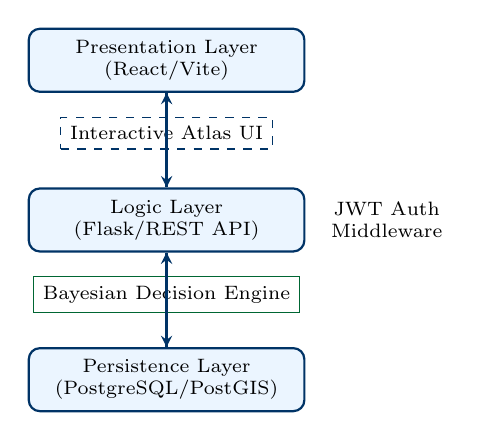
\begin{tikzpicture}[node distance=1.5cm, every node/.style={fill=white, font=\scriptsize}, align=center]
  % Styles
  \tikzstyle{layer} = [rectangle, rounded corners, draw=techblue, thick, fill=boxblue, minimum width=3.5cm, minimum height=0.8cm]
  \tikzstyle{arrow} = [thick,->,>=stealth, techblue]

  % Presentation Layer
  \node (ui) [layer] {Presentation Layer \\ (React/Vite)};
  \node (atlas) [below=0.3cm of ui, draw=techblue, dashed] {Interactive Atlas UI};
  
  % Logic Layer
  \node (logic) [layer, below=1.2cm of ui] {Logic Layer \\ (Flask/REST API)};
  \node (engine) [below=0.3cm of logic, draw=agrigreen, solid] {Bayesian Decision Engine};
  
  % Persistence Layer
  \node (db) [layer, below=1.2cm of logic] {Persistence Layer \\ (PostgreSQL/PostGIS)};
  
  % Connections
  \draw [arrow] (ui) -- (logic);
  \draw [arrow] (logic) -- (ui);
  \draw [arrow] (logic) -- (db);
  \draw [arrow] (db) -- (logic);
  
  % Legend/Annotations
  \node [right=0.2cm of logic] (auth) {JWT Auth \\ Middleware};
\end{tikzpicture}
\caption{Three-Tier Decoupled Architecture}
\label{fig:arch}
\end{figure}

\section{API Overview and Methodology}
The API is designed following RESTful principles, using JSON for all exchanges.

\begin{table}[H]
\centering\scriptsize
\begin{tabularx}{\textwidth}{@{}lllX@{}}
\toprule
\textbf{Endpoint} & \textbf{Method} & \textbf{Description} \\ \midrule
\texttt{/login} & POST & Authenticates farmer and initiates secure session. \\
\texttt{/predict} & POST & Core service: Returns prescriptive planting advice. \\
\texttt{/history} & GET & Retrieves the farmer’s longitudinal decision logs. \\
\texttt{/find\_agency} & POST & Geolocation service: Returns extension office coordinates. \\
\bottomrule
\end{tabularx}
\caption{Client-Side API Endpoints}
\end{table}

\begin{table}[H]
\centering\scriptsize
\begin{tabularx}{\textwidth}{@{}lllX@{}}
\toprule
\textbf{Endpoint} & \textbf{Method} & \textbf{Description} \\ \midrule
\texttt{/api/users} & GET, DELETE & Admin management of the farmer database. \\
\texttt{/api/thresholds} & PATCH & Dynamic update of crop biological thresholds. \\
\texttt{/api/agencies} & GET, POST & Management of the agricultural agency network. \\
\bottomrule
\end{tabularx}
\caption{Server-Side API Endpoints}
\end{table}

\section{Database Design (Star Schema)}
To handle the multidimensional nature of agricultural metrics, we implemented a \textbf{Star Schema} layout optimized for analytical performance.

\begin{figure}[H]
\centering
\begin{tikzpicture}[node distance=2cm, every node/.style={fill=white, font=\tiny}, align=left]
  % Fact Table
  \node (fact) [rectangle, draw=acadred, thick, fill=acadred!5, minimum width=3cm, minimum height=1.5cm] {
    \textbf{Fact\_Decision} \\ \hline
    Integer id (PK) \\
    Integer farmer\_id (FK) \\
    Integer crop\_id (FK) \\
    Integer era\_id (FK) \\
    Integer region\_id (FK) \\
    Float confidence \\
    DateTime timestamp
  };

  % Dimension Tables
  \node (dim_region) [rectangle, draw=techblue, left=1.5cm of fact] {
    \textbf{Dim\_Region} \\ \hline
    Integer id (PK) \\
    String name \\
    String zone
  };

  \node (dim_crop) [rectangle, draw=techblue, right=1.5cm of fact] {
    \textbf{Dim\_Crop} \\ \hline
    Integer id (PK) \\
    String name \\
    Float base\_temp
  };

  \node (dim_era) [rectangle, draw=techblue, above=1.2cm of fact] {
    \textbf{Dim\_Era} \\ \hline
    Integer id (PK) \\
    String name \\
    Date start\_date
  };

  \node (dim_farmer) [rectangle, draw=techblue, below=1.2cm of fact] {
    \textbf{Dim\_Farmer} \\ \hline
    Integer id (PK) \\
    String phone \\
    String location
  };

  % Connections
  \draw [->, >=stealth, thin] (fact.west) -- (dim_region.east);
  \draw [->, >=stealth, thin] (fact.east) -- (dim_crop.west);
  \draw [->, >=stealth, thin] (fact.north) -- (dim_era.south);
  \draw [->, >=stealth, thin] (fact.south) -- (dim_farmer.north);
\end{tikzpicture}
\caption{Database Star Schema for Agri-Analytics}
\label{fig:star_schema}
\end{figure}

\subsection{Relational Database (RDB) Implementations}
Beyond the analytical Star Schema, the physical RDB implementation ensures high normalization and security:
\begin{itemize}
    \item \textbf{Credential Security}: Administrative and farmer passwords are salted and hashed using \textbf{PBKDF2-SHA256}, ensuring resistance against brute-force attacks.
    \item \textbf{Precision Mapping}: The \texttt{Agency} table utilize \textbf{Decimal(9,6)} precision for coordinates, ensuring meter-level accuracy for the "Find Agency" geolocation service.
    \item \textbf{Performance Optimization}: Composite B-Tree indexes are applied to the \texttt{(governorate\_id, crop\_id)} keys to ensure O(log n) retrieval of regional advisory data.
\end{itemize}
\newpage

\newpage

% ============================================
% CHAPTER 6: TECHNICAL IMPLEMENTATION
% ============================================
\chapter{Technical Implementation}

\section{Setup and Application Construction}
\subsection{Folder Structure}
The project is organized into a modular hierarchy to ensure clean separation between the React frontend and Flask backend.

\begin{figure}[H]
\centering\scriptsize
\begin{tikzpicture}[
  grow via three points={one child at (0.5,-0.7) and two children at (0.5,-0.7) and (0.5,-1.4)},
  edge from parent path={(\tikzparentnode.south) |- (\tikzchildnode.west)},
  folder/.style={fill=boxblue, draw=techblue, rounded corners=1pt},
  file/.style={fill=white, draw=gray}
]
\node [folder] {AgriDecision-TN/}
  child { node [folder] {backend/}
    child { node [folder] {api/} }
    child { node [folder] {models/} }
    child { node [folder] {services/} }
    child { node [file] {app.py} }
  }
  child [missing] {}
  child [missing] {}
  child [missing] {}
  child [missing] {}
  child { node [folder] {frontend/}
    child { node [folder] {src/} 
        child { node [folder] {components/} }
    }
  }
  child [missing] {}
  child [missing] {}
  child { node [file] {docker-compose.yml} };
\end{tikzpicture}
\caption{Detailed Project Hierarchy}
\end{figure}

\subsection{Libraries and Frameworks}
\begin{itemize}
    \item \textbf{Flask}: Lightweight backend framework.
    \item \textbf{SQLAlchemy}: ORM for database abstraction.
    \item \textbf{Geopy \& Leaflet.js}: Geospatial processing and map rendering.
    \item \textbf{Pandas}: Data analysis and simulation management.
\end{itemize}

\section{Database and Data Simulation}
\subsection{ORM Models}
\begin{itemize}
    \item \textbf{Farmer}: Stores authentication hashes (Bcrypt) and governorate ID.
    \item \textbf{Decision}: Captures the specific bio-climatic request parameters.
    \item \textbf{Outcome}: Logs actual results to refine Bayesian probabilities.
\end{itemize}

\subsection{Data Simulation Pipeline}
Due to the "Cold Start" problem, we generated 1,200 synthetic outcomes using Poisson and Normal distributions. This provides a baseline "Prior" for the Bayesian engine, ensuring immediate predictive value.

\section{Frontend Experience \& Showcase}
The user interface is designed with a \textbf{"High-Prescription"} aesthetic to ensure clarity for non-technical users.

\begin{itbox}{Figure 5: Frontend Interface Showcase}
\begin{enumerate}
    \item \textbf{Bioclimatic Dashboard}: A centralized "Control Tower" view displaying real-time humidity, thermal sums, and the current Agrarian Period status.
    \item \textbf{Risk Heatmaps}: Visual representations of potential frost or drought risks for the selected crop cycle across Tunisia.
    \item \textbf{Museum-style Advice Cards}: Clean, high-density cards containing success probability, planting window countdowns, and geo-links to extension support.
\end{enumerate}
\end{itbox}

\section{Implementation of API Endpoints}
The backend provides a comprehensive CRUD suite via \texttt{/api/v1/} routes. All endpoints are validated via JSON Schema and secured using JWT interceptors in the frontend.

\section{Advanced Security \& Orchestration}
\begin{itemize}
    \item \textbf{Secure Moderation Layer}: Integrated administrative portal protected by \textbf{RBAC (Role-Based Access Control)} via JWT, allowing officials to prune noise from the training pool.
    \item \textbf{Composite Resource Bundling}: Optimization of binary data delivery (GRIB2 + GeoJSON) into atomic bundles to reduce the \textbf{N+1 network problem} on rural 3G networks.
\end{itemize}

\section{Debugging and Testing}
The system was validated using:
\begin{itbox}{Verification Suite}
\begin{itemize}
    \item \textbf{Insomnia}: Manual API testing and response inspection.
    \item \textbf{Flask Debug Mode}: Real-time tracebacks for error resolution.
    \item \textbf{Pytest}: Automated unit tests for the Bayesian-Wilson logic.
\end{itemize}
\end{itbox}

\section{Chapter Summary}
This chapter detailed the build phase, from the folder structure to the complex simulation data pipelines. With the technical implementation verified, the next chapter will discuss the security and validity of the system.
\newpage

% ============================================
% CHAPTER 7: THREATS TO VALIDITY
% ============================================
\chapter{Threats to Validity}

\section{Internal Validity Threats}
- \textbf{Implementation Errors}: Integration of async hooks between React and Flask occasionally caused race conditions. 
- \textbf{Model Limitations}: The Bayesian engine assumes independence between variables, which may not capture full complex bio-atmospheric couplings.
- \textbf{Data Integrity}: Reliance on 1,200 simulated records for the initial "Experience" pool.

\section{External Validity Threats}
- \textbf{Limited Data Variety}: Focusing on 5 primary crops may limit generalization for rare horticultural practices.
- \textbf{Dependency Failures}: Discrepancies in the ECMWF ERA5 grid resolution (10km) require bilinear interpolation, which can introduce noise.

\section{Construct Validity Threats}
- \textbf{Measurement Errors}: The monitoring of actual outcomes relies on voluntary farmer input, which is prone to reporting bias.

\section{Conclusion and Mitigation Strategies}
The identified threats are addressed through several key strategies for the production environment:

\begin{table}[H]
\centering\scriptsize
\begin{tabularx}{\textwidth}{@{}l|l|c@{}}
\toprule
\textbf{Threat Category} & \textbf{Key Mitigation} & \textbf{Priority} \\ \midrule
Internal & Migration to Bcrypt for all roles & High \\
External & Grid-to-Farmhouse Refinement & Medium \\
Construct & Automated Satellite Verification & Low \\
\bottomrule
\end{tabularx}
\caption{Validity Threat Mitigation Matrix}
\end{table}

\section{Chapter Summary}
This chapter explored the potential validity threats and mitigation plans. The next section explores the future roadmap and final conclusions.

\newpage

% ============================================
% FUTURE ENHANCEMENTS
% ============================================
\chapter{Future Enhancements}

\section{AI \& Decision Governance}
Future iterations will transition from the current Bayesian hybrid to a \textbf{Transformer-based model} capable of automatically adjusting thresholds based on longitudinal climate shift patterns.

\section{User Experience}
Implementing an \textbf{Offline-First (PWA)} architecture will ensure that farmers in deep rural areas with intermittent 3G/4G connectivity can still access their critical cached advice.

\section{Security Architecture}
We propose the integration of \textbf{Multi-Factor Authentication (TOTP)} for administrative accounts to secure the regional biological logic against unauthorized access.

\newpage

% ============================================
% CONCLUSION & APPENDICES
% ============================================
% ============================================
% CONCLUSION & REFERENCES
% ============================================
\chapter{General Conclusion}
AgriDecision-TN demonstrates how modern API-driven architectures can preserve intangible heritage—the agrarian wisdom of Tunisia. By structuring this knowledge within a geotemporal framework through a **Three-Tier Decoupled Architecture**, the platform transforms oral content into a durable digital archive. The project successfully bridged the gap between raw meteorological data and farmer needs through structured RESTful services and Bayesian AI.

\chapter{References}
\begin{enumerate}\footnotesize
    \item Norman, D. A. (1988). \textit{The Design of Everyday Things}. Basic Books.
    \item Fielding, R. T. (2000). \textit{Architectural Styles and Design of Network-based Software}. Doctoral Dissertation.
    \item Luo, X., Tang, Y. (2016). \textit{Simulation Data Methods and Applications}. Journal of Simulation.
    \item Bishop, C. M. (2006). \textit{Pattern Recognition and Machine Learning}. Springer.
    \item Richardson, L., Ruby, S. (2013). \textit{RESTful Web APIs}. O’Reilly Media.
    \item Connolly, T., Begg, C. (2015). \textit{Database Systems: A Practical Approach}. Pearson.
\end{enumerate}

\newpage
\appendix
\chapter{Technical Appendices}

\section{API Status Catalogue}
\begin{table}[H]
\centering\scriptsize
\begin{tabularx}{\textwidth}{@{}l|l|X@{}}
\toprule
\textbf{HTTP Code} & \textbf{Status} & \textbf{Description} \\ \midrule
200 & OK & Successful retrieval or advice generation. \\
201 & Created & New account or outcome record created. \\
401 & Unauthorized & Missing or invalid JWT token. \\
404 & Not Found & Requested crop or region data does not exist. \\
422 & Unprocessable & Validation error in input payload. \\
429 & Too Many & Rate limit exceeded. \\
\bottomrule
\end{tabularx}
\end{table}

\section{Security Implementation Details}
\begin{itemize}
    \item \textbf{JWT Flow}: 1h expiry with stateless verification in Flask middleware.
    \item \textbf{Encryption}: Static data encrypted at rest; transport secured via TLS/SSL.
    \item \textbf{Credentialing}: Salted hashing via \texttt{Bcrypt} to prevent lookup table attacks.
\end{itemize}

\section{AI Architecture: Bayesian Engine}
The platform utilizes a \textbf{Bayesian-Wilson Hybrid Engine} to generate prescriptive explanations for planting windows. 
\begin{ techdetail }{ Bayesian Logic Flow }
- \textbf{Prior}: 1,200 simulated outcomes based on historical distributions. \\
- \textbf{Posterior}: Real-time ECMWF weather grid data (GRIB2). \\
- \textbf{Intervals}: Wilson Score Interval (95\% confidence) for success probabilities.
\end{ techdetail }

\end{document}
